
\begin{summary}
We present an expectation-maximization algorithm to solve the \emph{inverse problem} for iterated function systems (IFS): the task of fitting a fractal model to a given dataset. An IFS is defined by a small number of maps on $\mathbb{R}^H$, the IFS's \emph{components}. A point is sampled from the IFS by starting with some initial point and applying a sequence of randomly chosen components. The central idea of our algorithm is to treat this sequence as a latent variable. If we are given such a \emph{code} for each point in the data, we know which points should map to one another under each transformation of the IFS, allowing us to reconstruct the components. Given the components, we can easily assign codes each point. Iterating these two steps provides us with a basic algorithm to fit an IFS model to data.
\end{summary}

In the previous section, we met statisticians faced with graph data, and saw the envy they feel for their colleagues with tabular data who know exactly how to slice and dice their bitstrings. Their data is \emph{symmetrical under translation}: slide the bitstring a fixed number of bits to the left or right, and the data looks the same. Not exactly the same, of course, but the probability distribution over the instance we are looking at remains fixed.

As we saw, in analysing graphs we have very little idea of how to move our data so that the part we're looking at stays the same. Motifs provide one solution: if we look at one motif instance, and move the graph around so that we are facing another instance of the same motif, we have achieved a kind of symmetry. Not as clean as our smug colleagues with their tabular data, but it's a start at least.

There is, however, another kind of symmetry in graph data that is rarely used in tabular data: \emph{symmetry under re-scaling}. This principle is commonly used implicitly: no researcher actually has access to the entire web-graph. What is commonly used is a subgraph of the whole, extracted by crawling links on the web. All research using such datasets makes the implicit assumption that conclusions drawn on the basis of this subgraph also hold for the whole. A subgraph, some times much smaller than the full object under study, is assumed to be similar to the whole set.

This assumption may seem reasonable, but it can have some far reaching consequences. For instance, if the subgraph is like the whole in every respect, is a subgraph of the subgraph also like the subgraph, and thereby like the whole? Can the whole dataset be split in increasingly smaller sections that are all scaled down copies of the whole? The result is a fractal: a shape determined entirely by its self-similarity.

Fractals models have been popular since the seventies, when mathematicians and physicists began to realize that they could explain jagged, irregular features like coastlines, clouds and trees. Object that had been proving increasingly difficult to analyze with  classical Euclidean geometry. One problem that has always held back fractal analysis, however, is the inverse problem: we know how to draw pictures of a fractal model, but how to reconstruct the model given the picture?

To simplify the task, we investigate the problem in the domain of tabular data: we consider fractal datasets as points drawn independently from some self-similar distribution on a $d$-dimensional Euclidean space. We show that the inverse problem can be efficiently solved with Expectation-Maximization methods.

\section{Introduction}
What constitutes a fractal is not precisely defined. \footnotemark There are, however, three properties that are common to most objects that are described as fractals. First, there is \textbf{self similarity}: a part is a scaled down copy of the whole. See for instance the Sierpinski triangle (fig. \ref{figure:codes}). It consists of three triangular shapes which are scaled down copies of itself. Second, fractals tend to posess \textbf{infinitely fine structure}. 'Zooming in' reveals ever finer detail. In the case of the Sierpinski triangle, we will see the same shape recurring again and again, but other fractals like the Mandelbrot set reveal a great variety of shapes.
Finally, fractals tend to have \textbf{non-integer dimension}. The Sierpinski triangle, for example, has a Hausdorff dimension of $1.58$. 
 
\begin{figure}[b!]
  \centering
  \begin{subfigure}[b]{0.48\textwidth}
    \includegraphics[width=\textwidth]{./images/sierpinski-codes.pdf}
    \caption{}
    \label{fig:sierpinski-codes}
  \end{subfigure}  
  \hspace{0.015\textwidth}
  \begin{subfigure}[b]{0.48\textwidth}
    \includegraphics[width=\textwidth]{./images/code-construction.pdf}
    \caption{}
    \label{fig:code-construction}
  \end{subfigure}

  \caption{\small (a) Codes of length three on the Sierpinski triangle and the subsets they code for. (b) The construction of a subset from its code.}
  \label{figure:codes}
\end{figure}

Since the name fractal was coined in the 1970s, fractals have been seen as a potential model for many natural phenomena. Mandelbrot put it as follows in the \emph{The Fractal Geometry of Nature} \cite{mandelbrot1982fractal}:

\begin{quotation}
\small
\noindent Clouds are not spheres, mountains are not cones, coastlines are not circles, and bark is not smooth, nor does lightning travel in a straight line.
\end{quotation}

Fractal geometry has been used in many fields, including physics \cite{mandelbrot1984fractals}, geology \cite{cheng1997multifractal}, biology \cite{goldberger1992fractal} and economics \cite{turiel2003multifractal}.

One of the greatest problem with fractal analysis has always been the difficulty of finding a fractal model for a given set of data. It may be visually clear that a cloud or a coastline `looks' fractal, and we may be able to determine that it has a non-integer dimension, but how do we get from a dataset to a model? How do we determine the parameters of a fractal-generating model that lead to this particular dataset? Current approaches tend to rely on evolutionary algorithms \cite{deliu1991genetic}. Such algorithms take a long time, and it can be difficult to get them to converge to precise parameter values, even if the dataset itself is sampled from a fractal model.
Other approaches are highly domain-specific, such as fractal image compression \cite{hart1996fractal}. Some interesting results have been also been derived from the method of moments \cite{rinaldo1994inverse} and sampling random transformations from the data \cite{hart1997similarity}, but so far these have not led to a practical algorithm. 

\footnotetext{Mandelbrot originally defined it as a set whose topological dimension differs from its Hausdorff dimension, but retracted this definition, stating that he preferred the word to be not precisely defined.}

A very popular fractal model is the iterated function system (IFS). Many fractals, like the Sierpinski gasket, the Koch curve and the Menger sponge can be seen as IFSs. We will use the following definition:
\begin{definition}
An \emph{Iterated Function System} of order $K$ and dimension $H$ is a pair $(\{f_k\}, \{w_k\})$ of $K$ \emph{components} $f_k$ with $K$ associated \emph{weights} $w_k$. Each component is is a function $f_k: \R^H \to \R^H$, and each weight is a nonnegative scalar, with $\sum_i w_i = 1$. 
\end{definition}
In this paper, all components are similitudes: ie. $f_k$ is defined by a scalar $s_k$, a rotation matrix $R_k$ and a translation vector $t_k$:
\[
f_k(x) = s_kR_k x + t_k \p
\]
The definition can be extended to functions of any kind on metric spaces \cite{hutchinson2000deterministic}, but this formulation is sufficient for our purposes. 

The IFS determines a probability distribution on $\R_H$ in the following way. Let $p_0$ be some initial distribution on $\R^H$, whose support is a compact set, and let $D$ be some nonnegative integer. Let  $x_0 \sim p_0$. Let $x_1 \sim \sum_k  w_k f_k(x_0)$, that is, the distribution on $x_1$ is a mixture of the distribution on $x_0$ as transformed by the components. Let  $x_2 = \sum_k w_k f_k(x_1)$, and so on until $x_D$.

There are two basic properties to of IFSs. First, the distribution on $x_D$ converges with increasing $D$. We call the distribution it converges to the \emph{limit distribution}. Second, the limit distribution is independent of the choice of $p_0$. Thus, we can take the weights and components as \emph{parameters} that determine a distribution, and we can evaluate the IFS to high $D$ to approximate this ditribution. For formal statements of these properties and their proofs we refer the reader to \cite{hutchinson2000deterministic}. 

We can now frame the fractal inverse problem as a problem of statistical parameter estimation: we would like to find the IFS for which the probability of of the data under its limit distribution is maximal. The algorithm we describe is based on the following ideas:
\begin{itemize}
  \item Since the initial distribution doesn't matter, we can choose what we like. We choose the standard multivariate Normal (MVN) distribution $\cN_0$. The benefit of this choice is that every affine transformation of an MVN is itself an MVN. Thus, no matter how high we set $D$, the resulting distribution will always be a mixture of MVNs. 
  \item We assume that each point in the dataset was the result of a sequence of applications of the components of the model. We cast this sequence---called a \emph{code} hereafter---as a latent variable in our model. Each code $c$ determines an \emph{endpoint distribution}, and each endpoint distribution is an MVN $\cN_c$.
  \item  Given the IFS that generated our data, it is a simple matter to find the most likely code for each point $x$. Conversely, if we know the most likely code for each datapoint, we can determine which points in the dataset should map to one another, under a particular component $f_k$. This correspondence allows us to reconstruct $f_k$.    
\end{itemize}

We make the correspondences in the last point probabilistic: instead of assigning each point its most likely code, we compute a \emph{responsibility} that each possible component takes for the point. This is the posterior probability of the component given the point: $p(c \mid x) \propto p(x \mid c) p(c)$, where $p(x\mid c) = N_c(x)$ and $p(x) = \prod_{s \in c} w_s$. This is the \emph{expectation} step of the algorithm. The \emph{maximization} step, optimizing the IFS model given these probabilities is detailed in the body of the paper. 

Note that finding a code corresponding to a particular endpoint can be counter-intuitive, as the first component applied determines the location at the smallest scale, and the last component applied determines the location at the largest scale. Figure~\ref{figure:codes} provides an illustration.

We show in Section~\ref{section:experiments} that our algorithm quickly reconstructs known fractals, such as the Sierpinski gasket and the Koch curve. We also apply the algorithm to some datasets sampled from images, and some natural data of higher dimension, showing that, while there are no IFSs to perfectly capture these images, the self similarity in the model does often allow a better fit than a simple mixture of MVNs.

\subsection{Preliminaries}
\paragraph{Measures and transformations} Let $\{x_i\}_{i\in[1,N]}$, $x_i\in\R^H$ be our dataset. Let $X$ be the $N\times H$ matrix with $x_i$ as its columns. All vectors are column vectors.  

Let $1_L$ be the length-$L$ vector with $1$ at all indices. Such vectors are useful tools in matrix notation: for instance, the sum of the elements of the $K \times L$ matrix $M$ can be expressed as ${1_K}^T M 1_L$, while its marginal vectors are $({1_K}^T M)^T$ and $M 1_L$. Let $0_L^j$ be the length-$M$ vector with element $j$ $1$ and all others $1$. This vector functions as a row- or column-selector, eg. $X 0^j_N = x_i$.

Let $v(X)$ be a probability distribution with $X \subseteq \R^H$. Let $f_{t, A}(x) = Ax + t$ be an invertible affine transformation represented by a vector $t$ and a matrix $A$. Then the transformation of $v$ by $f_{t, A}$ is defined by the relation $f_{t, A}(v)(X) = v({f_{t, A}}^{-1}(X))$. Let $v(x)$ be the density function of  the measure $v$ (with respect to the Lebesgue measure). Then the density function of the measure $f_{t, A}(v)$ is $f_{t, A}(v)(x) = |A^{-1}| v({f_{t, A}}^{-1}(x))$.

A multivariate normal distribution (MVN) on $\R^H$ is determined by a mean $\mu \in \R_H$ and a covariance matrix $\Sigma \in \R^{H\times H}$. Its probability density function is:
\[
\cN(x \mid \mu, \Sigma) = (2\pi)^{-\frac{H}{2}}|\Sigma|^{-\frac{1}{2}} \exp \left [-\frac{1}{2} \left \| (x-\mu)^T\Sigma^{-1}(x-\mu) \right\|^2\right] 
\]
We will call the MVN with $\mu = 0$, $\Sigma = I_H$ the standard multivariate normal distribution, or $\cN_0$. A \emph{spherical MVN} has $\Sigma = sI$ for some scalar $s$. Let $x$ be random variable with $x \sim \cN(\mu, \Sigma)$, then $f_{t, A}(x) \sim \cN(t + A\mu, A\Sigma A^T)$. 

A \emph{rotation matrix} $R$ is a matrix with $R_R = I$ and $|R| = 1$. A \emph{similitude} (or rigid transformation) on $\R^H$ is a transformation defined by a rotation matrix $R \in \R^{H\times H}$, a translation vector $t \in \R^H$ and uniform scaling $s \in R$: $f_{t, R, s}(x) = sRx + t$. 
The inverse of a similitude is also a similitude: ${f_{s, R, t}}^{-1}(x) = f_{\frac{1}{s}, R^T, -\frac{1}{s}R^Tt}(x)$.

$f_{s, R, t}(\cN_0)$ is a spherical MVN with mean $t$ and covariance $s^2I$. Transforming a generic spherical MVN by a similitude can be cast as the transformation of $\cN_0$ by two similitudes:
\begin{align}
f_{t, R, s}(\cN_{t_0, {s_0}^2 I})(x) &= f_{t, R, s}(f_{t_0, R_0, s_0}(\cN_0))(x) \notag \\
&=  (2\pi)^{-\frac{H}{2}} ({ss_0})^{-H} \exp \left[- \frac{1}{2{s_0}^2s^2}\left\| x - (s R t_0 + t)\right \|^2\right] \label{line:inverse}
\end{align}
\paragraph{The EM Algorithm} \cite{dempster1977maximum}
Let $p(X\mid Z, \theta)$ be probability distribution with parameters $\theta$ and latent variables $z$. In the most common oexample of the EM algorithm, $p$ is a mixture of MVNs: $\theta$ contains the parameters of $K$ MVNs together with a weight $w_k$ for each. $Z$ is a matrix whose rows $z_i$ determine which component is responsible for $x_i$: ie. if component $k$ is responsible, then $Z_{ik}$ is 1 and all other elements of row $i$ are 0.

The maximum likelihood parameters for a dataset $X$ are determined by 
\[
\argmax_{\theta} \ln p(X|\theta) = \argmax_{\theta} \ln \sum_Z p(X|Z, \theta)p(Z) 
\]
where the sum is over all possible values of $Z$. The value inside the sum is the \emph{complete-data likelihood} $p(X, Z\mid \theta)$. In the mixture-of-MVNs example, there are $K^N$ possibilities for $Z$, making this sum intractable for practical data. 
 
The intuition behind EM is to optimize $\theta$ with respect to our best guess for $Z$ and vice versa. Let $\theta^\text{old}$ be our current best guess for the parameters. We first optimize $p(Z\mid X, \theta^\text{old})$, the posterior on the latent variables. Note that, in the MVN example, we can represent this as an $N\times K$ matrix $Z$ with $Z_{ij} = p(j\mid x,\theta) = N^\text{old}_j(x) w_j$. These are known as the \emph{responsibilities}.

We then determine the expectation of the logarithmic complete-data likelihood under  our posterior $p(Z|X, \theta^\text{old})$ as a function of $\theta$.
\[
Q(\theta) = \sum_Z p(X|Z, \theta^\text{old})p(Z) \ln p(X, Z \mid \theta)
\]  
Note that the complete-data likelihood is now inside the logarithm. We optimize this \emph{$Q$-function}, with respect to $\theta$:
\[
\theta^\text{new} = \argmax_\theta Q(\theta)\p
\]
 The computation of the matrix $Z$ is know as the \emph{expectation} step and the computation of $\theta^\text{new}$ is known as the \emph{maximization} step. The EM algorithm iterates the two steps until the parameters converge.

\section{The IFS model}

\begin{figure*}[t]
  \center
  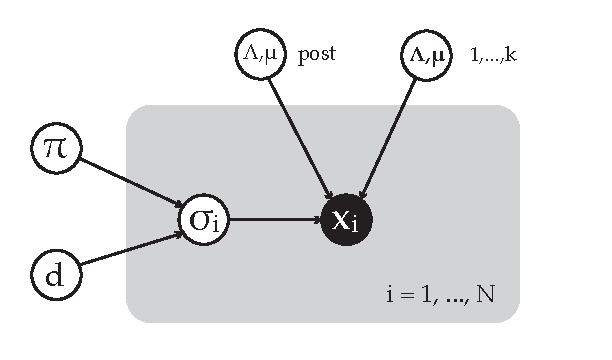
\includegraphics[width=0.7\textwidth]{./images/factor-graph.pdf}
  \caption{A graphical model, illustrating the components of the IFS model. The gray box is a plate, representing a repetition of the nodes inside the box for each datapoint. The black node represents the observed data.}
  \label{figure:ifs-diagram}
\end{figure*}

The complete IFS model is illustrated in Figure~\ref{figure:ifs-diagram}. It consists of:
\begin{description}
\item[the depth  priors $v$] The number of times the IFS is iterated for each point. $v$ is a vector representing a categorical distribution on $[0,D]$, from which the length of the code $c$ is sampled.
\item[the component weights $w$] This is a vector of $K$ non-negative real values, with $\sum_k w_k = 1$. Each weight determines the probability of its associated component being chosen at each iteration of the IFS.
\item[the components $f_k = \{s_k, R_k, t_k\}$] $K$ similitudes. 
\item[The post-transformation $s_p, R_p, t_p$] The parameters a single \emph{post-transformation}. This transformation is applied once to all sampled points.
\item[The code $c_i$] An ordered sequence $c_i = \langle c_{i1}, \ldots, c_{id} \rangle$. Each element of the code is an integer in $[1,K]$ representing a component. 
\item[The data $x_i$] This is the point after the post-transformation is applied: ie. the observed data.
\end{description}

To sample a point $x_i$ from this model we first sample a depth $d$ with $p(d=a) = v_a$. We then sample a sequence $c_j$ of $d$ components $c_{i1}, \ldots, c_{id}$ with each $c_ji \in [1,K]$ chosen independently with $p(c_{ji} = a) = w_a$. We then create the composite function $f = f_p \circ f_{c_{j1}} \circ \ldots \circ f_{c_{jd}}$ and sample $x$ from $f(\cN_0)$. Equivalently, we can sample $x_0$ from $\cN_0$ and apply the components prescribed by $c_i$ in series, and then apply $f_p$.

Giving the model a variable depth has several advantages. First, it makes the model a generalization of good fall-back models. With $v_0 = 1$, the model becomes a spherical multivariate Gaussian. With $v_1 = 1$, the model becomes a mixture of spherical Gaussians.\footnotemark Since each point has its own depth, the full model is a mixture over all these models, and the deeper IFS models. If the data is not self similar, or only partially self similar (like an IFS model with outliers), the lower depth parts of the mixture can account for this.

The variable depth also allows the EM search a `gentle start'. In the limit, most IFSs have a support with lower dimension than the embedding dimension of the data: ie. almost all of $\R^H$ has probability zero. This means that even if the model fits the source of the data perfectly, the slightest addition of noise will make the entire likelihood zero. It also means that a minute change in parameters can mean the difference between the maximum likelihood, and likelihood zero. In effect, for high values of $d$, the fitness landscape becomes very jagged. 

The depth parameters provide an automatic defense: if such a drop occurs, the lower models, whose fitness landscape is smoother, automatically get a higher posterior, smoothing out the fitness landscape for the complete mixture. As the search converges to the correct model, the depth prior becomes more weighted towards the higher depths.

However, the variable depth also creates a problem when our data is not perfectly centered. If we transform an IFS, evaluated to depth $d$, by an affine transformation, the result is also an IFS. However, the resulting components depend on $d$. Imagine a dataset sampled from a Sierpinski gasket translated away form the origin. We have good models at every depth for this data, but their components are different. Only if the data is centered do the components coincide for all depths. This is desirable, because once the solution has converged to these components, we will see the higher depths gaining more weight. But how the data should be centered for the components to coincide differs from one IFS to another. This is the reason for the \emph{post-transform}: we learn a centered IFS, and transform it to the data.   

\footnotetext{To generalize to non-spherical MVNs and mixtures over non-spherical MVNs, the component family should be extended to positive definite affine functions. This extension is discussed in the conclusion.}

\section{The EM algorithm for IFS models}

We will use the notation $[1,K]^d$ to refer to the set of all length-$d$ codes. Let $[1,K]^{[a,b]} = \bigcup_{d \in [a,b]} [1,K]^d$. Thus, the set of all codes, including the empty code, is $[1, K]^{[0, D]}$. For every code $c_j$ in this set, we have 
\begin{align*} 
p(x \mid c_j) &= \cN(x \mid \mu_j, \Sigma_j) \\
p(c_j) &= p(d) \prod_i p(c_j) = v_{|c_j|}\prod_{i \in c_j} w_{i}
\end{align*}

Where $\mu_j$ is the mean corresponding to $f_j(\cN_0)$ with $f_j = f_p \circ f_{c_{j1}} \circ f_{c_{j2}} \circ \ldots \circ f_{c_{jd}}$, and $\Sigma_j$ is the covariance matrix $f_j(\cN_0)$.

\subsection{Expectation: the latent variables}

The responsibilities for an MVN mixture model are well-known. Let $M = |[1, K]^{[0, D]}|$ and let $P$ be an $N\times M$ matrix with: 
\[
P_{ij} = p(c_j \mid x_i) = \frac{p(x_i\mid c_j) p(c_j) }{\sum_{a \in [1,K]^{[0, D]}} p(x_i\mid c_a) p(c_a)} \p 
\]
We also define a specific matrix for each $f_k$ for purposes that will become clear in the next section. Let $M = |[1, K]^{[0, D-1}]|$, and let $P^k$ be an $N \times M$ matrix with: 
\[
P_{ij}^k = p(k.c_j \mid x_i) = \frac{p(x_i\mid k.c_j) p(k.c_j) }{\sum_{a \in [1,K]^{[0, D]}} p(x_i\mid c_a) p(c_a)} 
\]
where $k.c_j$ is the code $\langle k, c_{j1}, \ldots\rangle$. Note that this is a sub-matrix of $P$.

The size of these matrices will grow very fast with $D$, and most of its values will be practically indistinguishable from $0$ when normalized. For this reason, it may be advisable to set all but the largest values to $0$, and store the matrix in a sparse datastructure. For our experiments, such optimizations were not necessary.

\subsection{Maximization: the parameters}

Let $\theta^\text{old}$ be the model we used to compute the responsibilities. Our $Q$-function is:
\begin{align*}
Q(\theta) &= \sum_{i} p(z_i \mid x_i, \theta^\text{old}) \ln p(x_i \mid z_i, \theta) p (z_i \mid \theta) \\
     &= \sum_{i=1,j=1}^{N, M} P_{ij} \ln \cN_j(x) \;v_{|c_j|}\; \prod_{a\in c_j}w_a \,\,\, \text{with } M = |[1,K]^{[0,D]}|
\end{align*}

For clarity of notation, when optimizing for a certain subset of the parameters $q$ (such as the depths, weights or parts of the components) we will write $Q(q)$, and omit any terms that are constant with respect to $q$. We may also omit any constant multiplier of the whole function.

To find the optimal depth we solve $\partial Q(v)/\partial v$, using a Lagrange multiplier to enforce that $v$ sums to one, which gives us:
\[
\hat v_d = \frac{p_d}{\sum_i p_i} \,\,\text{with } p_d = \sum_{j: |c_j| = d} P_{ij}
\]

\paragraph{The components $f_k$ and weights $w_k$}

Even with the simplifications of the EM algorithm $Q$ is very difficult to optimize for $f_k$ and $f_p$. We must find $K$ maps and weights, and a post-transformation $f_p$, such that all the $M$ endpoint distributions, provide maximal likelihood to their assigned points. The problem is that each term in $Q$ is a complicated mix of multiple components.

To make the optimization of $Q$ practical, we simplify the task in two ways. First, we optimize $f_p$ and $(\{f_k\}, \{w_k\})$ separately, taking the parameters not being optimized from $F^\text{old}$. Let $Y = {f_p^\text{old}}^{-1}(X)$. Second, we simplify the $Q$ function as follows: 

\begin{align*}
Q(\{f_k\}, \{w_k\}) = \sum_k \sum_{i=1,j=1}^{N, M} & p(k.c_j \mid x, F^\text{old}) \ln f_p f_k(\cN_{j})(x_i) p^{\text{old}}(c_j) p(k)\\ & \hfill \text{with } M = |[1,K]^{[0, D-1]}|  \\
= \frac{1}{s^\text{old}_p}\sum_k \sum_{i, j} &P^k_{ij} \ln \left[ f_k(\cN_{j})(y_i) \; v_{|c_j|+1} p(c_j) \; w_k \right]\p
\end{align*}
We then \emph{approximate} all elements indexed by $j$, so that of all the transformations in each code, only the last one functions as an argument of $Q$. We approxiamte $\cN_j$ by computing it from the model $\theta^\text{old}$.

This gives us:
\begin{align*}
Q(f_k, w_k) &= \sum_{i, j} P^k_{ij} \ln f_k(\cN_j)(y_i) + \sum_{i, j} P^k_{ij} \ln w_k  
\end{align*}
Finding $w_k$ follows the same principle as the depths. We find:
\[
\hat w_k = p^k / \sum_{i} p^i \p
\]
with $p^k = {1_N}^TP^k1_M$, the sum of the elements of $P^k$.

If we isolate $f_k$, the problem is very similar to the one solved to construct the Coherent Point Drift (CPD) algorithm \cite{myronenko2010point}: transform a set of MVNs to maximize the likelihood of a dataset, with respect to responsibilities $P$. The main difference is that in our situation each component $N_j$ has its own variance. We follow the same approach, and as we shall see, the solutions for our problem are very similar to those of the CPD algorithm.

Using Equation~\ref{line:inverse} from the preliminaries, we can rewrite $Q(f_k)$ as a mixture of transformations of $\cN_0$:
\begin{align*} 
Q(s_k, R_k, t_k) &= - p^k H \ln s_k - \sum_{i, j} P^k_{ij} \frac{1}{2{s_j}^2{s_k}^2} \left\|y_i-t_k - s_k R_k t_j \right\|^2 
\end{align*}
where $s_j$, $R_j$ and $t_j$ are the parameters of the similitude $f_p \circ c_{j1} \circ \ldots \circ c_{jd}$. 

To find the optimal translation $t_k$, we solve $\partial Q(t_k)/\partial t_k = 0$, which yields, in matrix notation:
\begin{align*}
\hat t_k &= \frac{1}{p^k_z}YP^kZ1_M - \frac{1}{p^k_z}s_kR_kTZ{P^k}^T1_N = y^k - s_kR_k t^k
\end{align*} 
where $T$ is the matrix with $t_j$ as its columns, $Z = \text{diag}({s_1}^{-2}, \ldots, {s_M}^{-2})$ and ${p^k_z} = {1_N}^TP^kZ1_M$, the sum of the elements of the matrix $P^kZ$. Thus $\hat t_k$ is the difference between a weighted mean of the data $y^k$ and a weighted mean of the endpoint means $t_j$, scaled and rotated, where in both cases, the matrix  $P^kZ$, normalized to sum to one, determines the weights. Note that this is not a complete solution, since it still depends on $s_k$ and $R_k$. We can, however, plug $\hat t_k$ back into the $Q$-function to optimize for $R_k$.

Finding the optimal rotation matrix $R_k$ is more complex than simply finding the derivative and setting it equal to zero, since we have the constraint that $R_k$ is orthogonal and has determinant $1$. We use the technique described in \ref{myronenko2009closed} and \cite[Lemma~1]{myronenko2010point}. We first rewrite the objective function to the form $\text{tr}(A^TR_k)$, for some $A$. We fill in $\hat t_k$, and reduce to
\[ 
Q(R_k) = \text{tr}\left(\left[\ol{Y}^kP^kZ{\ol{T}^k}^T\right]^TR_k\right) 
\]
with 
\begin{align*}
\ol{Y}^k &= Y - y^k {1_N}^T\\
\ol{T}^k &= T^k - t^k {1_M}^T\\
\end{align*}
The optimal $R_k$ can be derived from the singular value decomposition (SVD) of $A=\ol{Y}^kP^kZ{\ol{T}^k}^T$: if $A = USV^T$, with $U$, $S$ and $V$ defined as normal for the SVD then we have $\hat R_k = U \;\text{diag} (1, \ldots, 1, |UV^T|)\; V^T$.

Finally, we derive the scaling parameter $s_k$ by filling in $\hat t_k$ and solving $\partial Q(S_k)/\partial s_k$. We get:

\begin{align*}
0 &= {s_k}^{-2}\;\text{tr}({\ol{Y}^k}^T\text{diag}(P^kZ1_M)\ol{Y}^k) + {s_k}^{-1}\;\text{tr}(\ol{T}^kZ{P^k}^T{\ol{Y}^k}^TR_k) -H p^k \p
\end{align*}
This is a quadratic polynomial in ${s_k}^{-1}$, which we can solve and invert to find $\hat s_k$.

\subsection{The post transform: $s_p$, $R_p$, $t_p$} Let $M = \left |[1,K]^{[0,D]}\right|$ The $Q$-function becomes:
\begin{align*}
Q(s_p, R_p, t_p) &= \sum_{i=1,j=1}^{N,M} p(c_j\mid x_i) \ln f_p(N_j)(x_i) p(c_j) \\
&= - p\ln s_p  - \frac{1}{2 {s_p}^2} \sum_{i, j} {s_j}^{-2} P_{ij} \| x - t_p -s_pR_pt_j \|^2 \\
\end{align*}
where $p = {1_N}^T P 1^M$ and $s_j$ and $t_j$ can be derived from the optimal components, as determined above. Note that $j$ now iterates over a larger set of codes.

The form of the $Q$ function is the same as the ones we used to derive the optimal components $s_k, R_k, t_k$. We follow the same derivations and get: 

\begin{align*}
\hat t_p &= \overline{x} - s_pR_p\overline{t}\\
\hat R_p &= U\;\text{diag}(1, \ldots, 1, |UV^T|)\;V^T & \text{with } USV = \text{svd}(A), A = \ol{X} P Z {\ol{T}}^T \\
\end{align*}
with 
\begin{align*}
\ol{x} &= ({1_N}^TPZ1_M)^{-1} XPZ1_M & & \ol{t} = ({1_N}^TPZ1_M)^{-1}TZP^T1_M\\
\ol{X} &= X - \overline{x}{1_N}^T & &\ol{T} = T - \overline{t} {1_M}^T\\
Z &= \text{diag}({s_1}^{-2}, \ldots, {s_M}^{-2})\\
\end{align*}

Finally, for $s_p$, we solve
\[
0 = {s_p}^{-2}\text{tr}(\ol{X}^T\text{d}(PZ1_M)\ol{X}) + {s_p}^{-1} \text{tr}(\ol{T}ZP^T\ol{X}^TR_p) - H p
\]

\begin{pseudo}[th]
\caption{One iteration of the EM algorithm for fitting a fractal model.}
{
Given: a dataset $X$, a number of components $K$, a maximum depth $D$. \\

$C \leftarrow [0,K]^{[0, D-1]}$, $M \leftarrow |C|$ \emph{\# the set of all codes of length up to $D$} \\
\emph{\# Expectation step}\\
$P_{ij} \leftarrow N_j(x_i) p(d) \prod_{c \in [1,K]^d} w_c$  \\ 
Normalize $P$ so that $P1_M = 1_N$ \\
\textbf{for each} $k \in [1,K]$: \\
\tab Let $P^k$ be the submatrix of $P$'s columns $j$ such that $c_{j1} = k$\\
\\
\emph{\# Maximization step} \\
$Y \leftarrow {f^\text{old}_p}^{-1}(X)$\\
for all $d$, $v_d \propto \sum_{j : |c_j| = d} P_{ij} $\\
\textbf{for each} $k \in [1,K]$: \\
\tab $w_k \leftarrow {1_N}^T P^k 1_M / \sum_i {{1_N}^T P^i 1_M}$\\
\tab $y^k \leftarrow {p^k}^{-1}YP^kZ1_M, \,\,\, t^k \leftarrow {p^k}^{-1} T^kZ{P^k}^T 1_N$\\
\tab $\ol{Y}^k \leftarrow Y + y^k{1_N}^T$, \,\,\, $\ol{T}^k \leftarrow T^k + t^k{1_M}^T$\\
\tab $Z \leftarrow \text{diag}({s_1}^{-2}, \ldots, {s_M}^{-2})$\\
\tab $U,S,V^T \leftarrow \text{svd}(\ol{Y}^kP^kZ{\ol{T}^k}^T)$\\ 
\tab $R_k \leftarrow U\;\text{diag}(1,\ldots,1,|UV^T|) V^T$ \\
\tab $s_k$: solve ${s_k}^{-2}\; \text{tr}({\ol{Y}^k}^T\text{d}(P^kZ1_M)\ol{Y}^k) + {s_k}^{-1}\;\text{tr}(\ol{T}^kZ{P^k}^T{\ol{Y}^k}^TR_k) - Hp^k= 0$ \\
\tab $t_k \leftarrow y^k - s_k R_k t^k$ \\

$C \leftarrow [0,K]^{[0, D]}$, $M \leftarrow |C|$\\
$X' \leftarrow X - \overline{x}{1_N}^T$, $T' \leftarrow T + \overline{t}{1_M}^T$\\
\tab $Z \leftarrow \text{diag}({s_1}^{-2}, \ldots, {s_M}^{-2})$\\
$U,S,V^T \leftarrow \text{svd}(X'PZ{T'}^T)$\\ 
$R_p \leftarrow U\;\text{diag}(1,\ldots,1,|UV^T|) V^T$ \\
$s_p$: solve ${s_p}^{-2}\text{tr}(X'PZ1_NX'+ T'Z{P}^T1_MT') - s_p^{-1} \text{tr}(ZP^T{x'}^TT') -Hp = 0$ \\
$t_p \leftarrow \overline{x} - s_pR_p\overline{t}$ \\
}
\end{pseudo}

\subsection{Dealing with singularities}

In the EM algorithm for MVN mixtures, there is a danger that the algorithm becomes stuck in a situation where one or more of the components do not have responsibility for any part of the data, or for only a single point. In this case, the covariance matrix for such components cannot be computed, and the algorithm must be reset in some way.

In the IFS algorithm a similar thing can happen, causing one or more of the matrices $P^k$ to become low-rank. In this case, the SVD decomposition required to find $R_k$ cannot be computed. When this happens, we use the following strategy: we remove the undetermined component, and for each one we \emph{split} one of the well-determined components. Let $f_a = (s_a, R_a, t_a)$ with weight be the well-determined component and $f_b$ be the singleton component. We resolve the situation by setting:
\begin{align*}
f_a \leftarrow (s_a, R_a, t_a + \epsilon_a)\\
f_b \leftarrow (s_a, R_a, t_a + \epsilon_b) 
\end{align*}
where $\epsilon_a, \epsilon_b$ are vectors with elements randomly drawn from $\cN(0, \sigma)$, where we use $\sigma = 0.001$ in all experiments. The weight $w_a$ is distributed equally over the components $f_a$ and $f_b$ and the weight vector is re-normalized.
 
The rationale is easiest to understand if we take $v_1=1$ and view the model as a mixture of Guassians. In that case, the well-determined components cover all the data. By splitting $f_a$, and adding some small noise, the points formerly `claimed' by $f_a$ will now be distributed approximately evenly between $f_a$ and $f_b$. 

A second trap is that the variance of the endpoint distributions can become so small that, even using logarithmic representation, the matrices $P^k$ become low-rank (ie, all entries are $0$) for certain components. If this happens, we reset the algorithm by approximating $P$  and all $P^k$: we still use the endpoint means $t_j$ from the model, but we place an MVN with a fixed standard deviation on each (we use the standard deviation 0.01 in all experiments) and re-compute the responsibilities under that model.

\section{Results}
\label{section:experiments}

To speed up the algorithm, we us a subsample (with replacement) from the data in all experiments. After each iteration (one expectation and one maximization step), we draw another sample. The sample size is always 250. We run the algorithm for 300 iterations, with maximum depth 5. In practice, it may be advisable to increase the sample size and the depth as the algorithm begins to converge, but for the sake of simplicity, we have kept the parameters fixed.

\subsection{Synthetic distributions}
\begin{figure*}
\begin{tabular}{c c c c c}
\hline
data & it. 20 & it. 40 & it. 250 & full depth \\
\hline
    \includegraphics[width=0.2\textwidth]{{./images/fractals/sierpinski/workspace/fractal/0/data}.pdf} & 
    \includegraphics[width=0.2\textwidth]{{./images/fractals/sierpinski/workspace/fractal/0/best/iteration.000020}.pdf} & 
    \includegraphics[width=0.2\textwidth]{{./images/fractals/sierpinski/workspace/fractal/0/best/iteration.000040}.pdf} & 
    \includegraphics[width=0.2\textwidth]{{./images/fractals/sierpinski/workspace/fractal/0/best/iteration.000299}.pdf} &
    \includegraphics[width=0.2\textwidth]{{./images/fractals/sierpinski/workspace/fractal/0/best/iteration.000299.deep}.pdf} \\ 
    \includegraphics[width=0.2\textwidth]{{./images/fractals/sierpinski-off/workspace/fractal/0/data}.pdf} & 
    \includegraphics[width=0.2\textwidth]{{./images/fractals/sierpinski-off/workspace/fractal/0/best/iteration.000020}.pdf} & 
    \includegraphics[width=0.2\textwidth]{{./images/fractals/sierpinski-off/workspace/fractal/0/best/iteration.000040}.pdf} & 
    \includegraphics[width=0.2\textwidth]{{./images/fractals/sierpinski-off/workspace/fractal/0/best/iteration.000299}.pdf} & 
    \includegraphics[width=0.2\textwidth]{{./images/fractals/sierpinski-off/workspace/fractal/0/best/iteration.000299.deep}.pdf} \\ 
	\includegraphics[width=0.2\textwidth]{{./images/fractals/koch2/workspace/fractal/0/data}.pdf} & 
    \includegraphics[width=0.2\textwidth]{{./images/fractals/koch2/workspace/fractal/0/best/iteration.000020}.pdf} & 
    \includegraphics[width=0.2\textwidth]{{./images/fractals/koch2/workspace/fractal/0/best/iteration.000040}.pdf} & 
    \includegraphics[width=0.2\textwidth]{{./images/fractals/koch2/workspace/fractal/0/best/iteration.000299}.pdf} & 
    \includegraphics[width=0.2\textwidth]{{./images/fractals/koch2/workspace/fractal/0/best/iteration.000299.deep}.pdf} \\ 
	\includegraphics[width=0.2\textwidth]{{./images/fractals/koch4/workspace/fractal/0/data}.pdf} & 
    \includegraphics[width=0.2\textwidth]{{./images/fractals/koch4/workspace/fractal/0/best/iteration.000020}.pdf} & 
    \includegraphics[width=0.2\textwidth]{{./images/fractals/koch4/workspace/fractal/0/best/iteration.000040}.pdf} & 
    \includegraphics[width=0.2\textwidth]{{./images/fractals/koch4/workspace/fractal/0/best/iteration.000299}.pdf} & 
    \includegraphics[width=0.2\textwidth]{{./images/fractals/koch4/workspace/fractal/0/best/iteration.000299.deep}.pdf} \\ 
	\includegraphics[width=0.2\textwidth]{{./images/fractals/sierpinski2/workspace/fractal/0/data}.pdf} & 
    \includegraphics[width=0.2\textwidth]{{./images/fractals/sierpinski2/workspace/fractal/0/best/iteration.000020}.pdf} & 
    \includegraphics[width=0.2\textwidth]{{./images/fractals/sierpinski2/workspace/fractal/0/best/iteration.000040}.pdf} & 
    \includegraphics[width=0.2\textwidth]{{./images/fractals/sierpinski2/workspace/fractal/0/best/iteration.000299}.pdf} & 
    \includegraphics[width=0.2\textwidth]{{./images/fractals/sierpinski2/workspace/fractal/0/best/iteration.000299.deep}.pdf} \\
\hline 
\end{tabular}  
  \caption{Results of EM search for known models. The red and blue boxes show the model: the post-transform maps the image frame onto the red box, and each component maps the red box onto a blue box. The bars in the side of the blue boxes show the weight of each component. The learning tasks, from top to bottom are: the Sierpinski gasket, the Sierpinski gasket with unequel weights, the Koch curve with 4 components, the Koch curve with two components and the Sierpinski gasket with two components.}
  \label{figure:synthetic}
\end{figure*}

Figure~\ref{figure:synthetic} shows the performance of the algorithm on four well known fractals: the Sierpinski gasket, a Sierpinski gasket with unequal weights, and two- and four-component versions of the Koch curve.

For each dataset we repeated the experiment 100 times and both the model with its learned mixture over depths, and what the IFS looks like when evaluated to infinite depth. \footnotemark We show the run that ended with a model with the greatest likelihood (on the training data). the end results of all runs are shown in the appendix. 

\footnotetext{Such data can be sampled using an algorithm known as the \emph{chaos game} \cite{barnsley2014fractals}.}
 
It is difficult to objectively quantify the number of trials that successfully converged to the required IFS. One may suggest testing the likelihood of the data under the learned model, to see if it is close to that of the target model, but the likelihood grows exponentially as the higher depths get greater weight (if the model is correct). This means that unless the algorithm finds the absolute correct model, the likelihoods of any learned model, correct or otherwise, will be much closer to one another than to the likelihood of the target model.  

We inspected the resulting models for each of the 100 runs visually to determine whether they were good approximations, and report the proportions here, with the proviso that these necessarily include some level of subjective judgment. The complete set of results for each experiment is reproduced in the appendix. 

We observe that the most difficult of these models appears to be two-component Koch curve. This is most likely due to the fact that the components of this model require an exact rotation. Compare this to the Sierpinski triangle, where each component can have a rotation of 0, 120 or 240 degrees, without changing the model.

\subsection{Non IFS data}

\begin{figure*}
\begin{tabular}{c c c c c}
\hline
data & it. 20 & it. 40 & final model & full depth \\
\hline
    \includegraphics[width=0.2\textwidth]{{./images/fractals/cloud/workspace/fractal/0/data}.pdf} & 
    \includegraphics[width=0.2\textwidth]{{./images/fractals/cloud/workspace/fractal/0/best/iteration.000020}.pdf} & 
    \includegraphics[width=0.2\textwidth]{{./images/fractals/cloud/workspace/fractal/0/best/iteration.000040}.pdf} & 
    \includegraphics[width=0.2\textwidth]{{./images/fractals/cloud/workspace/fractal/0/best/iteration.000299}.pdf} &
    \includegraphics[width=0.2\textwidth]{{./images/fractals/cloud/workspace/fractal/0/best/iteration.000299.deep}.pdf} \\ 
    \includegraphics[width=0.2\textwidth]{{./images/fractals/romanesco/workspace/fractal/0/data}.pdf} & 
    \includegraphics[width=0.2\textwidth]{{./images/fractals/romanesco/workspace/fractal/0/best/iteration.000020}.pdf} & 
    \includegraphics[width=0.2\textwidth]{{./images/fractals/romanesco/workspace/fractal/0/best/iteration.000040}.pdf} & 
    \includegraphics[width=0.2\textwidth]{{./images/fractals/romanesco/workspace/fractal/0/best/iteration.000299}.pdf} & 
    \includegraphics[width=0.2\textwidth]{{./images/fractals/romanesco/workspace/fractal/0/best/iteration.000299.deep}.pdf} \\ 
	\includegraphics[width=0.2\textwidth]{{./images/fractals/coast/workspace/fractal/0/data}.pdf} & 
    \includegraphics[width=0.2\textwidth]{{./images/fractals/coast/workspace/fractal/0/best/iteration.000020}.pdf} & 
    \includegraphics[width=0.2\textwidth]{{./images/fractals/coast/workspace/fractal/0/best/iteration.000040}.pdf} & 
    \includegraphics[width=0.2\textwidth]{{./images/fractals/coast/workspace/fractal/0/best/iteration.000299}.pdf} & 
    \includegraphics[width=0.2\textwidth]{{./images/fractals/coast/workspace/fractal/0/best/iteration.000299.deep}.pdf} \\ 
	\includegraphics[width=0.2\textwidth]{{./images/fractals/disc/workspace/fractal/0/data}.pdf} & 
    \includegraphics[width=0.2\textwidth]{{./images/fractals/disc/workspace/fractal/0/best/iteration.000020}.pdf} & 
    \includegraphics[width=0.2\textwidth]{{./images/fractals/disc/workspace/fractal/0/best/iteration.000040}.pdf} & 
    \includegraphics[width=0.2\textwidth]{{./images/fractals/disc/workspace/fractal/0/best/iteration.000299}.pdf} & 
    \includegraphics[width=0.2\textwidth]{{./images/fractals/disc/workspace/fractal/0/best/iteration.000299}.pdf} \\ 
	\includegraphics[width=0.2\textwidth]{{./images/fractals/sphere/workspace/fractal/0/data}.pdf} & 
    \includegraphics[width=0.2\textwidth]{{./images/fractals/sphere/workspace/fractal/0/best/iteration.000020}.pdf} & 
    \includegraphics[width=0.2\textwidth]{{./images/fractals/sphere/workspace/fractal/0/best/iteration.000040}.pdf} & 
    \includegraphics[width=0.2\textwidth]{{./images/fractals/sphere/workspace/fractal/0/best/iteration.000299}.pdf} & 
    \includegraphics[width=0.2\textwidth]{{./images/fractals/sphere/workspace/fractal/0/best/iteration.000299.deep}.pdf} \\
\hline 
\end{tabular}  
  \caption{Results of EM search for known models. The red and blue boxes show the model: the post-transform maps the image frame onto the red box, and each component maps the red box onto a blue box. The bars in the side of the blue boxes show the weight of each component. The learning tasks, from top to bottom are: the Sierpinski gasket, the Sierpinski gasket with unequel weights, the Koch curve with 4 components, the Koch curve with two components and the Sierpinski gasket with two components.}
  \label{figure:non-ifs}
\end{figure*}

Next, we try the model on five non-IFS datasets. The first three are derived from images of fractal phenomena: a Romanesco broccoli, a coast line, and the edge of a cloud, illuminated by sunshine. While these are fractals, they also contain a degree of noise, and a deterministic IFS is unlikely to capture them perfectly. The fourth dataset is sampled from a uniform distribution on the bi-unit disc. Unlike the square, the disc cannot be described as an IFS. However, at low depths, the model is forced to spend probability mass on the area outside the disc, so some balance must be struck. 

\subsection{Higher-dimensional data}

\begin{figure*}[htb]
  \centering
  \begin{subfigure}[b]{0.3\textwidth}
  	\includegraphics[width=\textwidth]{./images/fractals/abalone/likelihoods.pdf}
  	\caption{abalone}
  \end{subfigure}
  ~
  \begin{subfigure}[b]{0.3\textwidth}
  	\includegraphics[width=\textwidth]{./images/fractals/basketball/likelihoods.pdf}
  	\caption{basketball}
  \end{subfigure}
  ~
  \begin{subfigure}[b]{0.3\textwidth}
  	\includegraphics[width=\textwidth]{./images/fractals/galaxies/likelihoods.pdf}
  	\caption{galaxies}
  \end{subfigure}
  \caption{The negative log-likelihood of three models: the mixture of isotropic MVNs (iso), the mixture fo full MVNs (mog) and the IFS. Dots show the negative log-likelihood (ie. lower is better).}
  \label{figure:ifs-high}
\end{figure*}

In higher dimensions, it is difficult to establish whether a given dataset has fractal properties. Nevertheless, even if the data lacks such properties, the IFS model has certain attributes that may help it in modelling such data. First, the IFS can model distributions with lower dimension than the dimension of the euclidean space used to describe the data. This is something that a mixture of MVNs cannot do. Second, as we saw in the `disc' example above, the IFS can model hard edges in a distribution. And finally, the IFS can model many small areas with high density. 

To investigate the performance of IFS model, we select three suitable datasets with no particular expectation that they contain IFS-style self-similarity. These are: 
\begin{description}
\item[abalone \cite{nash1994population,lichman2013uci}] A dataset describing various properties of specimens of abalone (a marine mollusc). The class labels of the original dataset were discarded, leaving 4177 instances with 8 numeric features each. Available at \url{https://archive.ics.uci.edu/ml/datasets/Abalone}. 
\item[basketball] Each instance represents a year (from 1946 to 2004) that a player played for a given team. Each instance has 18 numeric attributes such as points scored and penalty minutes. The dataset contains around 19000 instances. Available from \url{databasebasketball.com}.
\item[galaxies] The 3D `coordinates' of around 18000 galaxies. Generated from the 2 Micron All-Sky Survey\cite{skrutskie2006two}, and transformed into Euclidean coordinates by John Huchra. Available at \url{https://www.cfa.harvard.edu/~dfabricant/huchra/seminar/lsc/}. 
\end{description}
All datasets we normalized so that each value for each dimension lay in the interval $[-1, 1]$. 

For each dataset, we learn a 3-component IFS, with a maximum depth of 7, sampling 500 points each iteration, for 300 iterations. We learn on a random selection of 50\% of the data, and compute the negative log-likelihood of the withheld data using the model of the last iteration. We repeat the experiment 50 times.

We compare against a mixture of isotropic (ie. spherical) MVNs and a mixture of MVNs with full covariance matrix. Note that the former is equivalent to our algorithm with the depth parameter fixed at $v_1 = 1$ and the post transform fixed at identity. The results are shown in Figure~\ref{figure:ifs-high}.

The most striking difference is that the IFS model shows much greater variability. In all three cases, there are parameters for which the IFS provides a better fit, but there is no guarantee that they will be found in a single run. While the IFS model should always be able to guarantee at least the same likelihood as the isotropic MVNs, we see here that the EM algorithm will, in some cases, return models worse than that.

Nevertheless, if the resources are available to perform multiple runs, the IFs model can provide a better fit than a mixture of Gaussians, a model with comparable parametrization.

\subsection{Complexity}
\begin{figure*}[htb]
  \includegraphics[width=\textwidth]{./images/fractals/timing.pdf}
  \caption{The time taken for a single iteration of the algorithm, separated into the expectation and the maximization step. For each value, the iteration was computed one hundred times. The graph shows the mean over these repetitions, the error bars show a 95\% confidence interval (ie. 1.96 times the standard error on both sides). Note the logarithmic axes on the second and third plot.}
  \label{figure:timing}
\end{figure*}

To give an indication of the complexity of the algorithm, we plot the time taken for a single expectation step and a single maximization step, against three variables: the size of the data sample, the dimension of the data, and the maximum depth.

In the first case, we sample the data from a three-dimensional standard normal distribution, use the Sierpinski gasket as an initial model, and compute one full iteration of the algorithm, measuring the time taken to complete the expecation and the maximization step. The depth is set to 5. 

For the second test, we  again sample from a standard normal distribution, but we vary its dimension from 1 to 50. The model is initialized at random using the method described earlier. The depth is set to 5.

For the final test we use the same procedure as for the first, but we fix the data size  at 250 and vary the depth from 0 to 10.
For all values, the experiments were repeated 100 times. The experiments we performed on a single machine with 8 Gigabyte of java heapspace and 2 1.80 Ghz Intel Xeon processors (E5-2650L). The code for a single iteration is single-threaded, and the matrix operations were not hardware accelerated. \footnotemark These options are still open to improve the algorithm's efficiency. The fast Gauss transform \cite{greengard1991fast,yang2003improved} may also speed up the computation of the expectation step.

\footnotetext{Specifically, we used the Apache Commons Mathematics library.}

Figure~\ref{figure:timing} shows the result. The strongest growth is in the depth, which is likely exponential, as the number of columns of $P$ alone grows exponentially in $D$. The growth in dimension looks to be polynomial first, up to around 20, and exponential afterwards. Why this is the case, and whether a polynomial growth for all dimensions is achievable requires further analysis.

\section{Discussion}

We have introduced a new algorithm for the induction of fractal models. To our knowledge this is the first such algorithm that does not use a general-purpose optimization technique like genetic algorithms. 

Similitudes were chosen as a nice balance between expressiveness and parameter complexity. More general function classes are certainly possible, although deriving the maximization step analytically may not be possible for these. For instance, if we allow generic, affine  functions, defined by a translation $t$ and a matrix $A$, we find a derivative of the form $\frac{\partial Q}{\partial A} |A^{-1}| + cA$. This is difficult, if not impossible to solve analytically, although if we restrict $A$ to be positive definite, we can see that the problem is convex, so that we can easily solve it numerically.

An alternative approach would be to use a variational Bayesian algorithm instead of an EM algorithm. If a variational algorithm exists for the desired function class, it should be straightforward to plug these into a general variational algorithm for iterated function systems. Such an approach would also avoid the problem of singularities, and it would allow some tuning of the algorithm through the selection of priors. We consider this a promising direction for future research.

Many natural fractal phenomena are not precisely captured by iterated functions systems. Coastlines trees and clouds are self-similar, but in a much more random manner than IFSs can describe. One solution takes the form of an extension to random iterated function sytems, as described in \cite{hart1996fractal}. Here, at each application the IFS is itself chosen at random from a distribution on IFSs. Another option would be to manually add domain knowledge about the data into the model, for instance specific knowledge about the development of clouds or the growth of trees. In both cases, we believe the EM algorithm provides a basic template for a solution: the main issue is that of finding the specific choices made inside the model to arrive at each point in the dataset. By casting this sequence of choices as a latent variable, and applying Bayes rule (either using EM or a variational approach), we divide and conquer: we cannot solve the problem as a whole, but we can find the latent variables given the parameters, and the parameters given the latent variables.

